\chapter{Investigating the sub-continental ancestry of ethnic minorities within the UK Biobank from sparse genotype data}
\label{chapterlabel3}

\section{Introduction}

From a genetic standpoint, the native British population is one of the most highly studied in the world, with many different studies sequencing or genotyping individuals from across the U.K (e.g. \cite{bycroft2018uk, Leslie2015, turnbull2018introducing, uk10k2015uk10k}). These studies have been aimed primarily at researching the genetic basis of disease. These data have also been used to investigate population history, substructure  and the relatiobship of different sub-populations in the U.K. to other European countries \cite{Leslie2015}.  

The U.K. is also an ethnically diverse country, at least 8m ethnic miority individuals living in the U.K. Groups of people from across the world have migrated to the U.K. at different periods in the previous 3 centuries, driven by the legacy of colonialism, the transatlantic Slave Trade and economic reasons. Despite this, the roughly 8 million ethnic minorities within the U.K. remain relatively understudied. For example, every one of the 27 papers in the GWAS catalog with "UK Biobank" in the title, and 2 others presently in the catalog curation queue, limited their analyses to EA subgroups varying described as "White British", "British" "European" "White European" "Caucasian" or "White" \cite{manolio2019using}. The primary reason for this is reasonable concerns over the confounding effect of population substructure within a cohort; retaining a more genetically homogeneous cohort is one strategy to mitigate this. 

Because of this, evidence is mounting that the results from GWAS studies, such as Polygenic Risk Scores, may not be transferrable to other populations if they have been conducted in cohorts of exclusively European individuals. The reasons for this is currently unclear, but it has been suggested that differences in LD structure may be the cause. Ethnic minorities may therefore miss out on the advances in healthcare driven by large-scale genomic projects. Understanding the population structure of ethnic minorities within the U.K. Biobank is an important step towards including a diversity of ancestries in GWAS. 

During the course of my PhD, I was fortunate to obtain the `Human Origins' dataset which, at the time of writing, is the most detailed dataset of genotype data from African individuals. Whilst the dataset contains individuals from across Africa, it contains particularly large numbers of individuals from South Africa (n=104), Cameroon (n=567) and Ghana (n=211), which are countries known to have contributed immigrants to the U.K. Therefore, this dataset is ideal for use as a reference panel to investigate the ancestry of ethnic minorities within the U.K. Biobank. In particular, I am interested in investigating the ancestry of individuals with recent African ancestry. 

As noted in the introduction, one issue is that a relatively small proportion of the SNPs overlap between the U.K. Biobank and Human Origins genotyping array; only 70,776 SNPs overlap, compared to a typical number between 500,000 and 700,000. Using a low number of SNPs in the analysis may reduce the power to infer accurate ancestry proportions, as there is less data points to compare populations with. Therefore, one option is to impute the non-overlapping SNPs using a reference panel. However, the effect of imputation on ChromoPainter-style analyses has yet to be fully investigated. It is possible that imputing a large number of positions may introduce biases, particularly towards populations which are present in the reference panel. Studies have shown repeatedly that genotypes in non-European individuals are imputed less accurately compared to European individuals. Accordingly, we can ask whether it is preferable to retain a smaller number of non-imputed SNPs or a larger number of imputed SNPs. 

This chapter will focus on two questions. Firstly, I am interested in relating the genetic variation of individuals in the U.K. Biobank with recent African ancestry to the populations in the Human Origins dataset. 


\section{Methods}

\subsection{Data access}

Access was obtained to study the UK Biobank dataset via UCL genetics institute. 

I first accessed the U.K. Biobank genotype data, consisting of 488,377 individuals genotyped at 784,256 genome-wide SNPs. Hereafter I will refer to this data as the `non-imputed' data. plink1.9 \cite{purcell2007plink} was used to convert the binary plink files to bgzipped vcf format. Strand inconsistencies between the UK Biobank and Human Origins dataset were identified using the gt-conform utilty from Beagle and any inconsistent positions removed. 

I also download U.K. Biobank data which has been imputed to approximately 96m SNPs. Data was imputed using the combined references of the Haplotype Reference Consortium (HRC) and UK10K haplotype resource. Full details of imputation can be found in the paper of McCarthy et al (2016) \cite{mccarthy2016reference}. The imputed data was downloaded and converted from .bgen to .vcf format using qctool. Strand inconsistencies between the UK Biobank and Human Origins dataset were identified using the gt-conform utilty from Beagle and any inconsistent positions removed.

\subsection{Data preparation - Human Origins}

To determine the ancestry patterns in U.K. Biobank individuals, it is necessary to compare them to reference dataset of individuals of known origin. As I am particularly interested in studying individuals with recent African ancestry, the Human Origins dataset (appendix A.20) is ideal for this purpose, as it contains many individuals from many different ethnic groups from across Africa. 


\begin{figure}[htp]
    \centering
    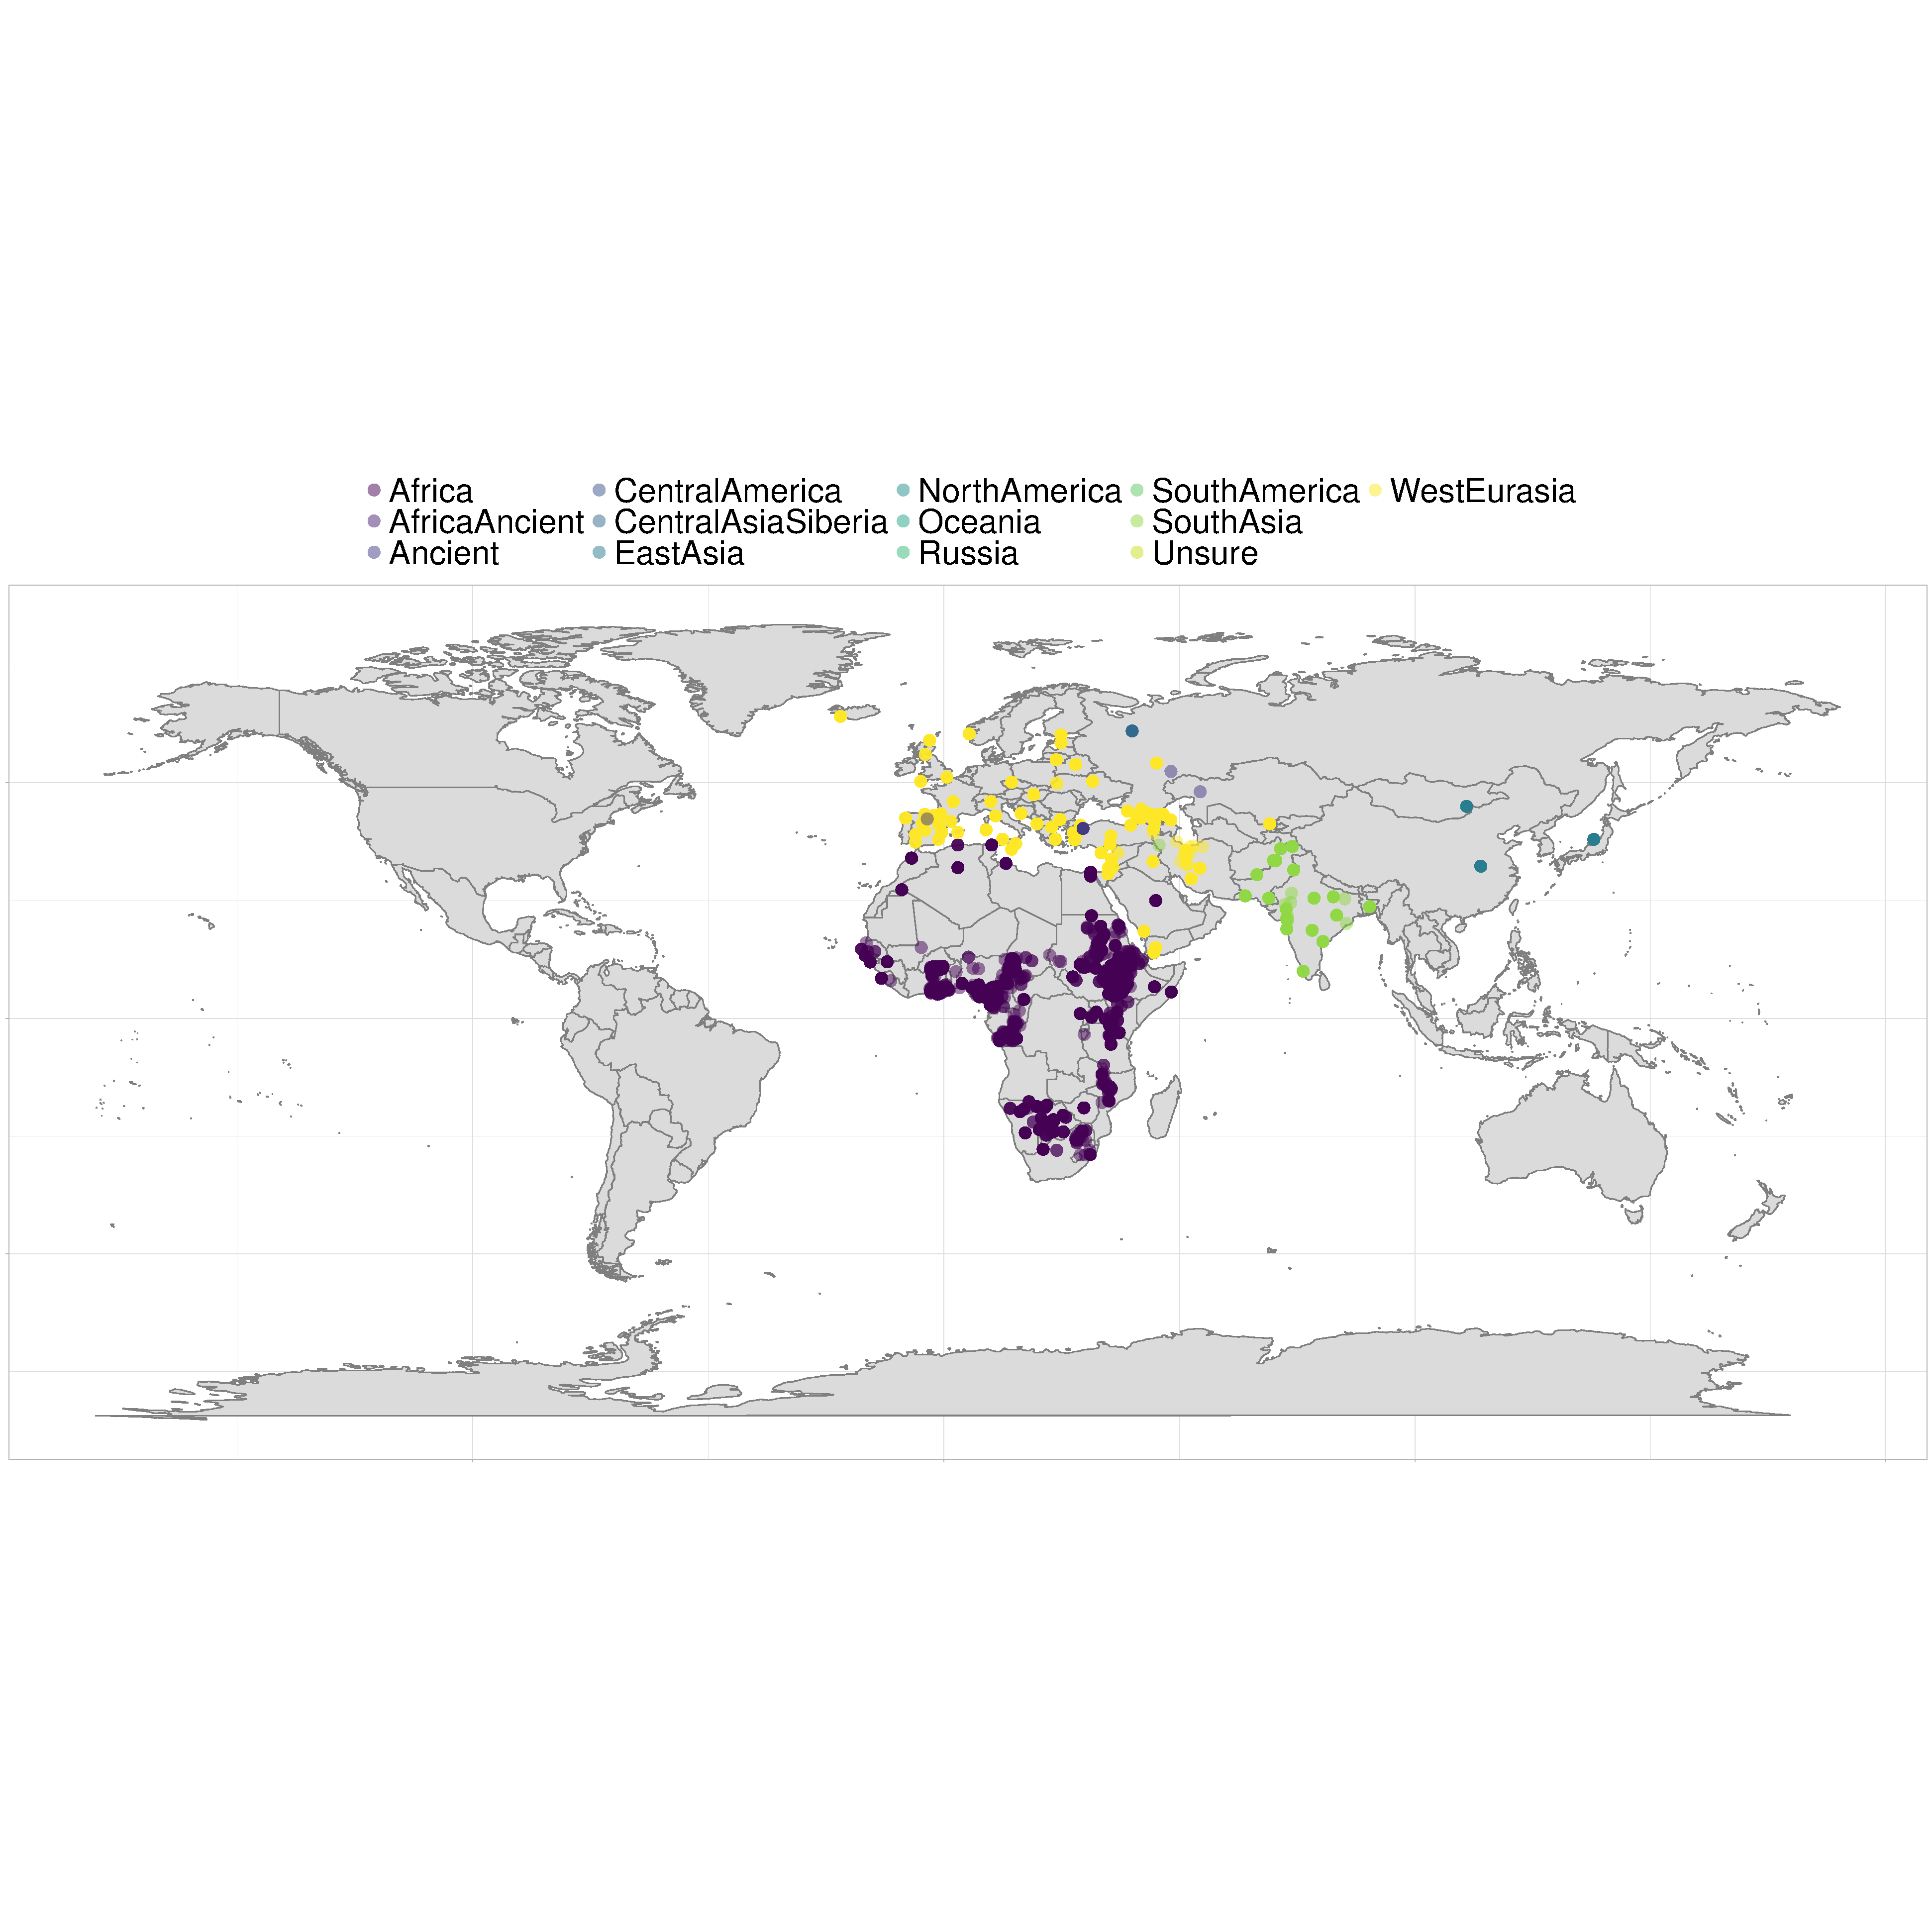
\includegraphics[width=1.0\textwidth]{../images/chapter3/HumanOriginsMap.pdf}
    \caption{Location of individuals present in the Human Origin dataset.}
    \label{fig:PCA_chunklengths_HumanOrigins_UKBiobank}
\end{figure}

\subsection{ADMIXTURE analysis}

Performing chromopainter analysis on the entire UK Biobank dataset (n=488,377 individuals) is currently computationally infeasible. Thus, I chose to analyse only those individuals with more than 50\% non-European ancestry. ADMIXTURE is a fast and accurate way to estimate continental-scale ancestry proportions.

I first LD pruned the non-imputed U.K. Biobank dataset using using the \texttt{plink --indep-pairwise 50 10 0.02} \cite{purcell2007plink}. This left a total of  70,776 bi allelic SNPs. I then subsetted the 1000 genomes dataset down to the 70,776 SNPs retained in the U.K. Biobank dataset and merged them using \texttt{bcftools merge}. Thus, I had a dataset containing all U.K. Biobank and 1000 genomes individuals. 

I ran a supervised ADMIXTURE analysis on each batch by using the \texttt{--supervised} command and fixing the 4 reference populations as GBR British, Nigeria Yoruba, Han Chinese and Gujarati Indian. The rest of the arguments were left to default.

\subsection{Data preparation - non imputed data}

It is necessary to merge datasets in order to jointly analyse them. I therefore merged the Human Origins and non-imputed U.K. Biobank datasets. I first identified which SNPs were common to both datasets and then subsetted both so that they contained only those SNPs, resulting in a total of 65,749 SNPs. I then merged the two datasets using \texttt{bcftools merge}. I only retained U.K. Biobank individuals if they had 50\% non-European ancestry or more, resulting in a total of 26,298 individuals. 

I phased the merged UK Biobank / Human Origins dataset using shapeit4 \cite{delaneau2018integrative}. I set \texttt{--pbwt-depth 8} and left all other parameters as default. The resulting vcf of phased haplotypes was converted to chromopainter format using a custom script.  

\subsection{Data preparation - imputed data}

Similarly to above, I needed to merge the imputed Biobank data with the Human Origins dataset. Again, I filtered both datasets to retain only SNPs which were common to both the datasets. The Human Origins and UK Biobank datsets were then merged using the \texttt{bcftools merge} command. The resulting merged dataset contained 493,407 individuals and 535,544 SNPs.

The merged dataset was then phased using shapeit4 \cite{delaneau2018integrative}, setting \texttt{--pbwt-depth 1} to increase speed at this large sample size. The phased output was converted to chromopainter output using a custom script.


\subsection{Imputation bias test}

Imputing variants in non-European individuals using a reference panel that is primarily composed of European individuals may lead to biased or inaccurate imputation. To explicitly evaluate this possibility, I performed a test using the Human Origins dataset.
 
To do this, I took the entire Human Origins dataset (5998 individuals and 560,420 SNPs) and submitted it to the Sanger Imputation Server, using the full Haplotype Reference Consortium (HRC) as a reference for phasing and imputation. This reference panel was chosen because it was the same one used for imputing the Biobank individuals.

I next subsetted the imputed Human Origins dataset down to SNPs present in the UK Biobank array , leaving 727,325 positions present in the imputed Human Origins dataset. I then performed an `all-v-all' painting, forming each target haplotype as a mosaic of all other haplotypes. I also performed an identical `all-v-all' painting of the same Human Origins dataset, but using the original set of SNPs where none had been imputed. 

Therefore, we had 2 coancestry matrices of identical structure, but one was generated using a majority of imputed SNPs and the other was generated using no imputed SNPs. 

I also performed SOURCEFIND analysis on both matrices. Individuals were grouped into populations and all populations were used as surrogates for each target population. Default parameters were used and each SOURCEFIND target was analysed for 2,000,000 MCMC iterations. Ancestry proportions and confidence intervals were estimated from the raw MCMC output using the Coda R library \cite{oro22547}.

\subsection{Chromopainter}

I performed 2 identical paintings using the imputed and non-imputed datasets. Both used all Human Origins samples as donors and all U.K. Biobank individuals as recipients. 

\subsection{SOURCEFIND}

\section{Results}

\subsection{ADMIXTURE}

I performed supervised ADMIXTURE on all 488,378 UK Biobank individuals in order to identify individuals with at least 50\% non-European ancestry. These individuals would then be carried forward to later analyses. In total, there were 8476, 2653, 9171 individuals with at least 50\% ancestry from Yoruba, Han Chinese and Gujarati reference populations respectively. 

To verify the accuracy of the ADMIXTURE results, I selected all individuals who self-identified as being either "Caribbean", "African" or "Black or Black British" (n=7527) and assessed the distribution of ADMIXTURE ancestry proportions, under the assumption that these individuals should contain more African than other kinds of ancestry. This was the case, with the mean proportion of African ancestry among these individuals being 0.85 (Fig. \ref{fig:African_Inds_proportions_ADMIXTURE}).

There is substantial variation in the ancestry proportions for those self-identified as being either "Caribbean", "African" or "Black or Black British" - proportions of Yoruban and British ancestry ranged from 0.00001 to 1, Han Chinese from 0.00001 to 0.53 and Gujarati from 0.759 to 0.00001, reflecting the diverse array of genetic ancestries that can fall under a given ethnic label. 


\begin{figure}[htp]
    \centering
    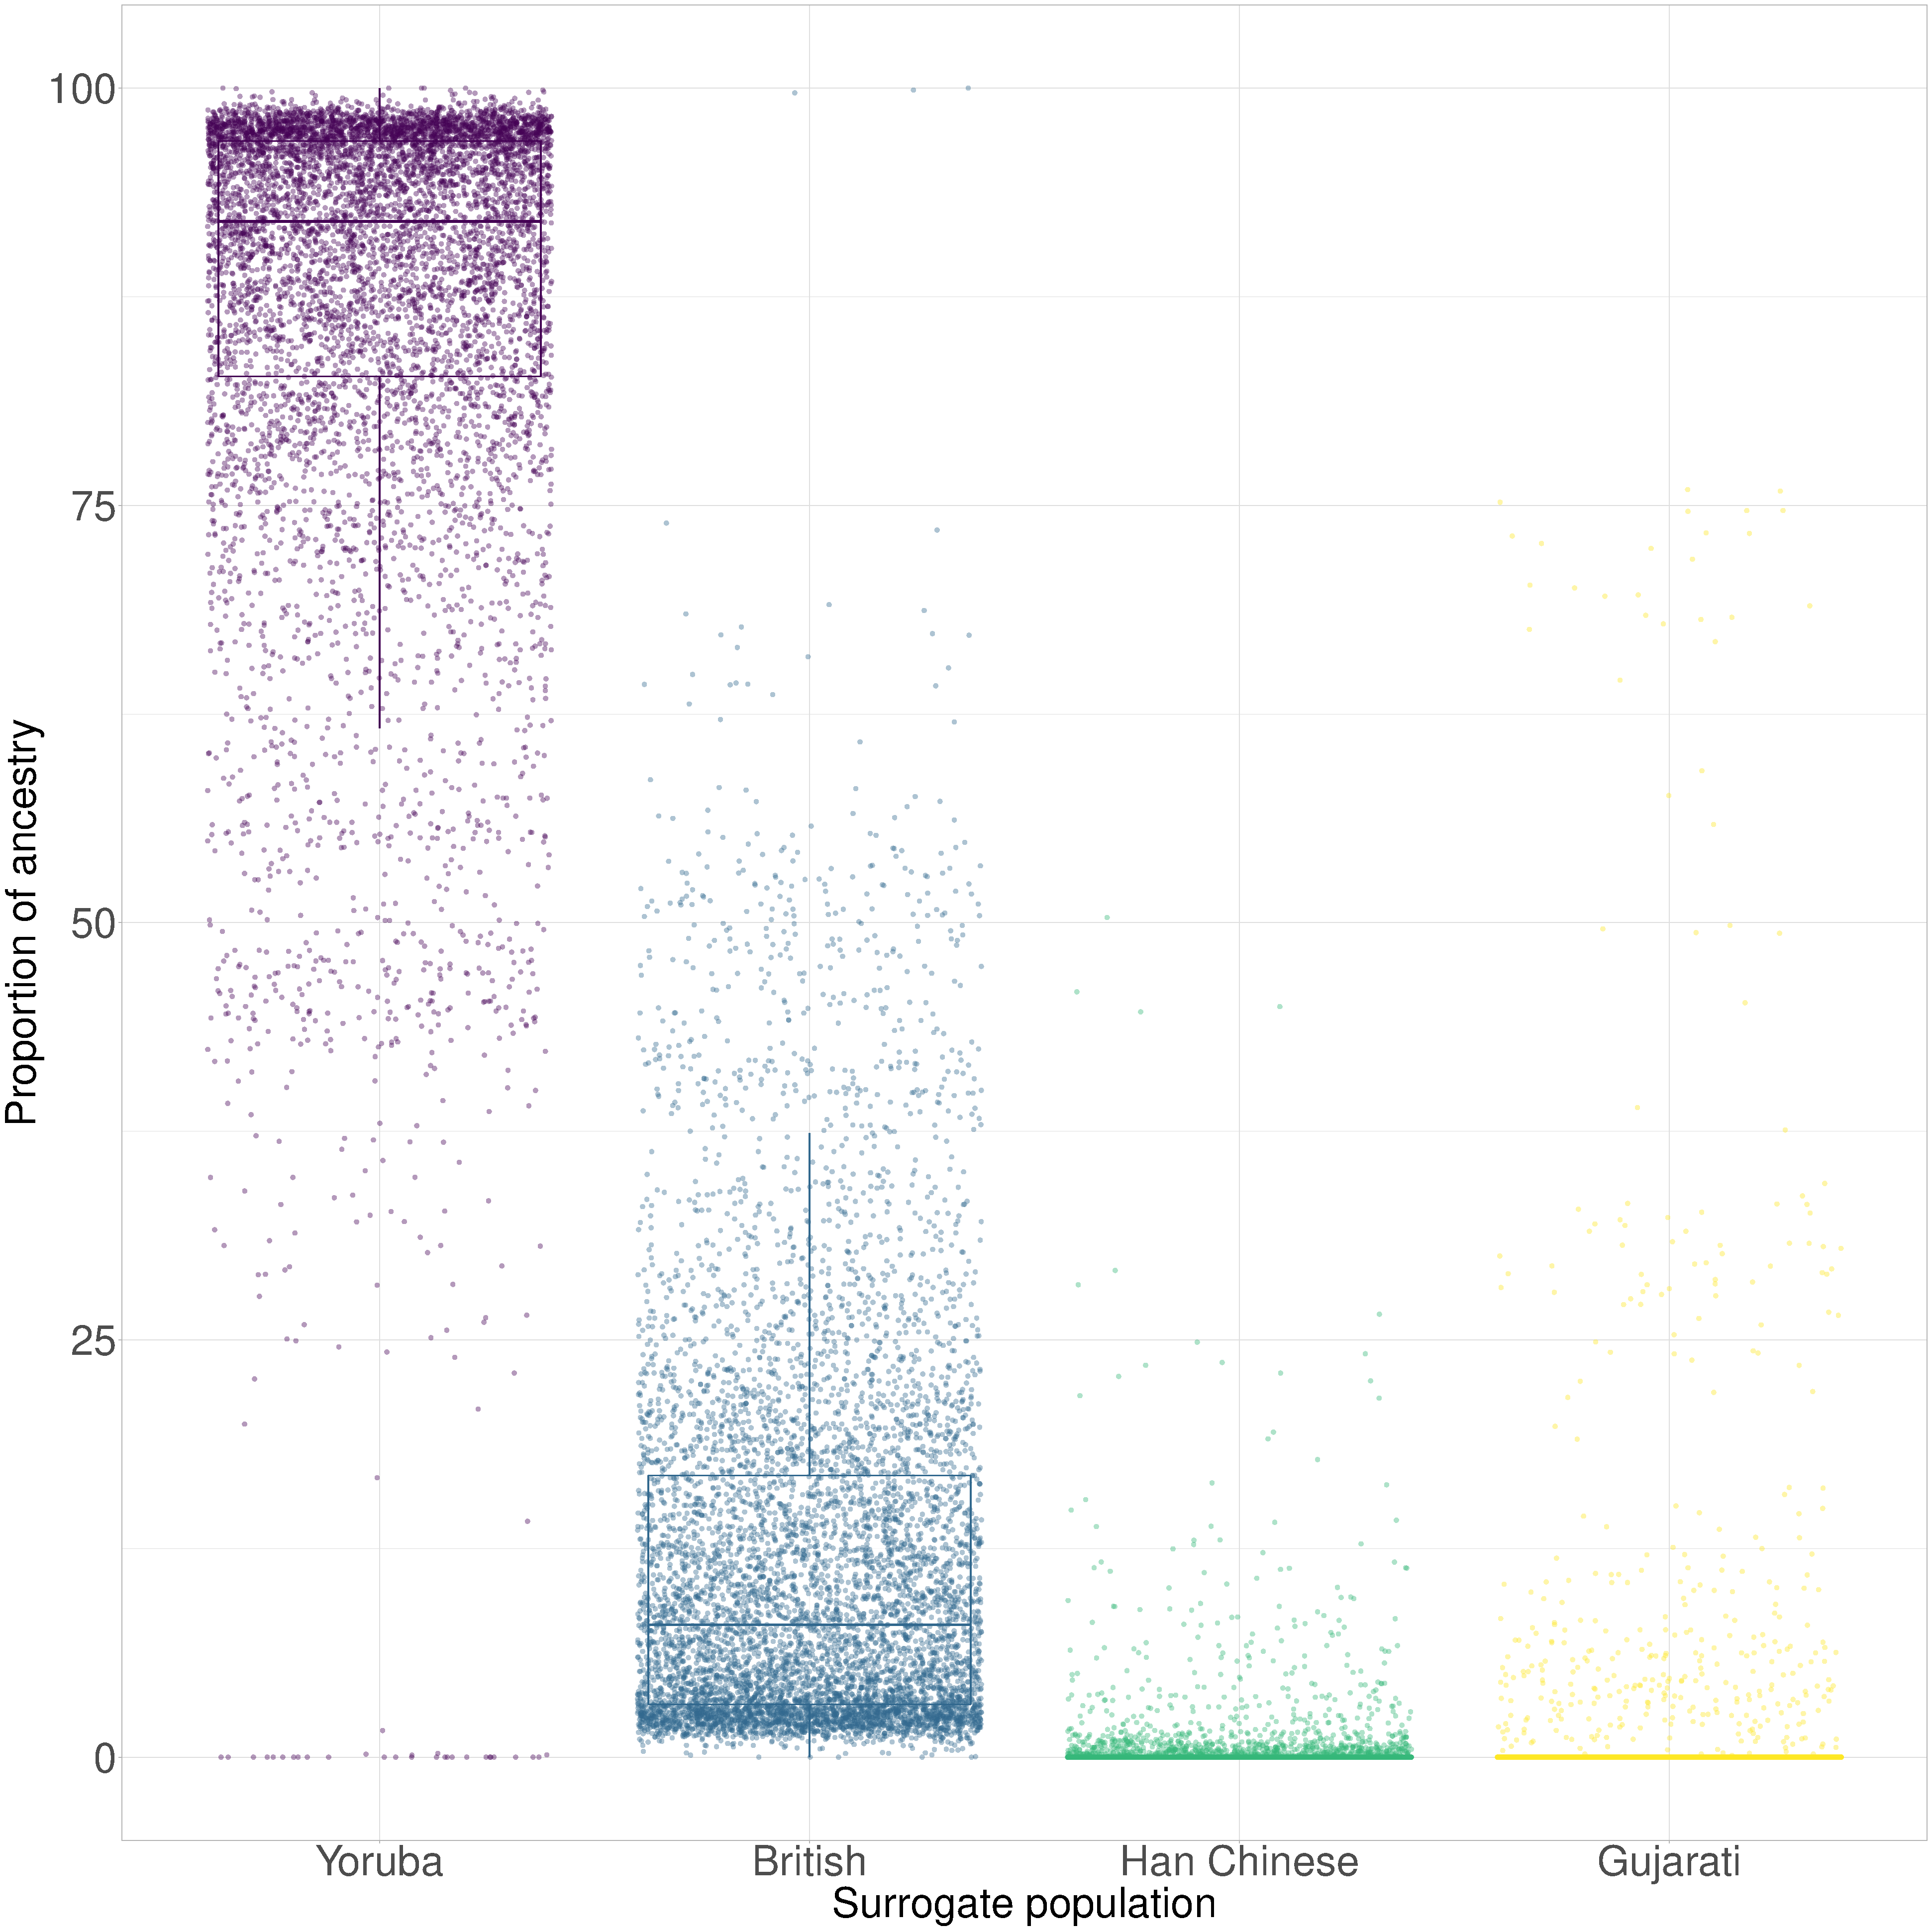
\includegraphics[width=1.0\textwidth]{../images/chapter3/African_Inds_proportions.pdf}
    \caption{Ancestry proportions inferred from supervised Admixture run (k=4) for all individuals who self identified as being either "Caribbean", "African" or "Black or Black British"}
    \label{fig:African_Inds_proportions_ADMIXTURE}
\end{figure}


\subsection{Chromopainter}

I performed a painting using all Human Origins individuals as donors and all U.K. Biobank individuals with at least 50\% African ancestry as recipients. 

Principle component analysis on this matrix reveals the general structure of the selected individuals, alongside the reference populations (Fig. \ref{fig:/PCA_chunklengths_HumanOrigins_UKBiobank}). Principle Component Analysis (PCA) can be performed on the co-ancestry matrix in order to visualise the underlying structure. As expected, PC1 seperates Africans from non-Africans and positions Europeans slightly closer to Africans than east-Asians, likely reflecting admixture into Africa from populations closer to Europeans than East-Asians. PC2 splits east and west Eurasians, again placing Africans closer to West than East Eurasians. 

Several notable patterns can be observed in the PCA. Firstly, whilst the Human Origins samples (green points) are more or less found entirely on 2 perpendicular lines, representing African and non-African samples, the UK Biobank samples are spread over the centre of the PCA. This reflects the different nature of the 2 datasets; the samples in Human Origins are not recently mixed, whereas many of the UK Biobank samples are.

\begin{figure}[htp]
    \centering
    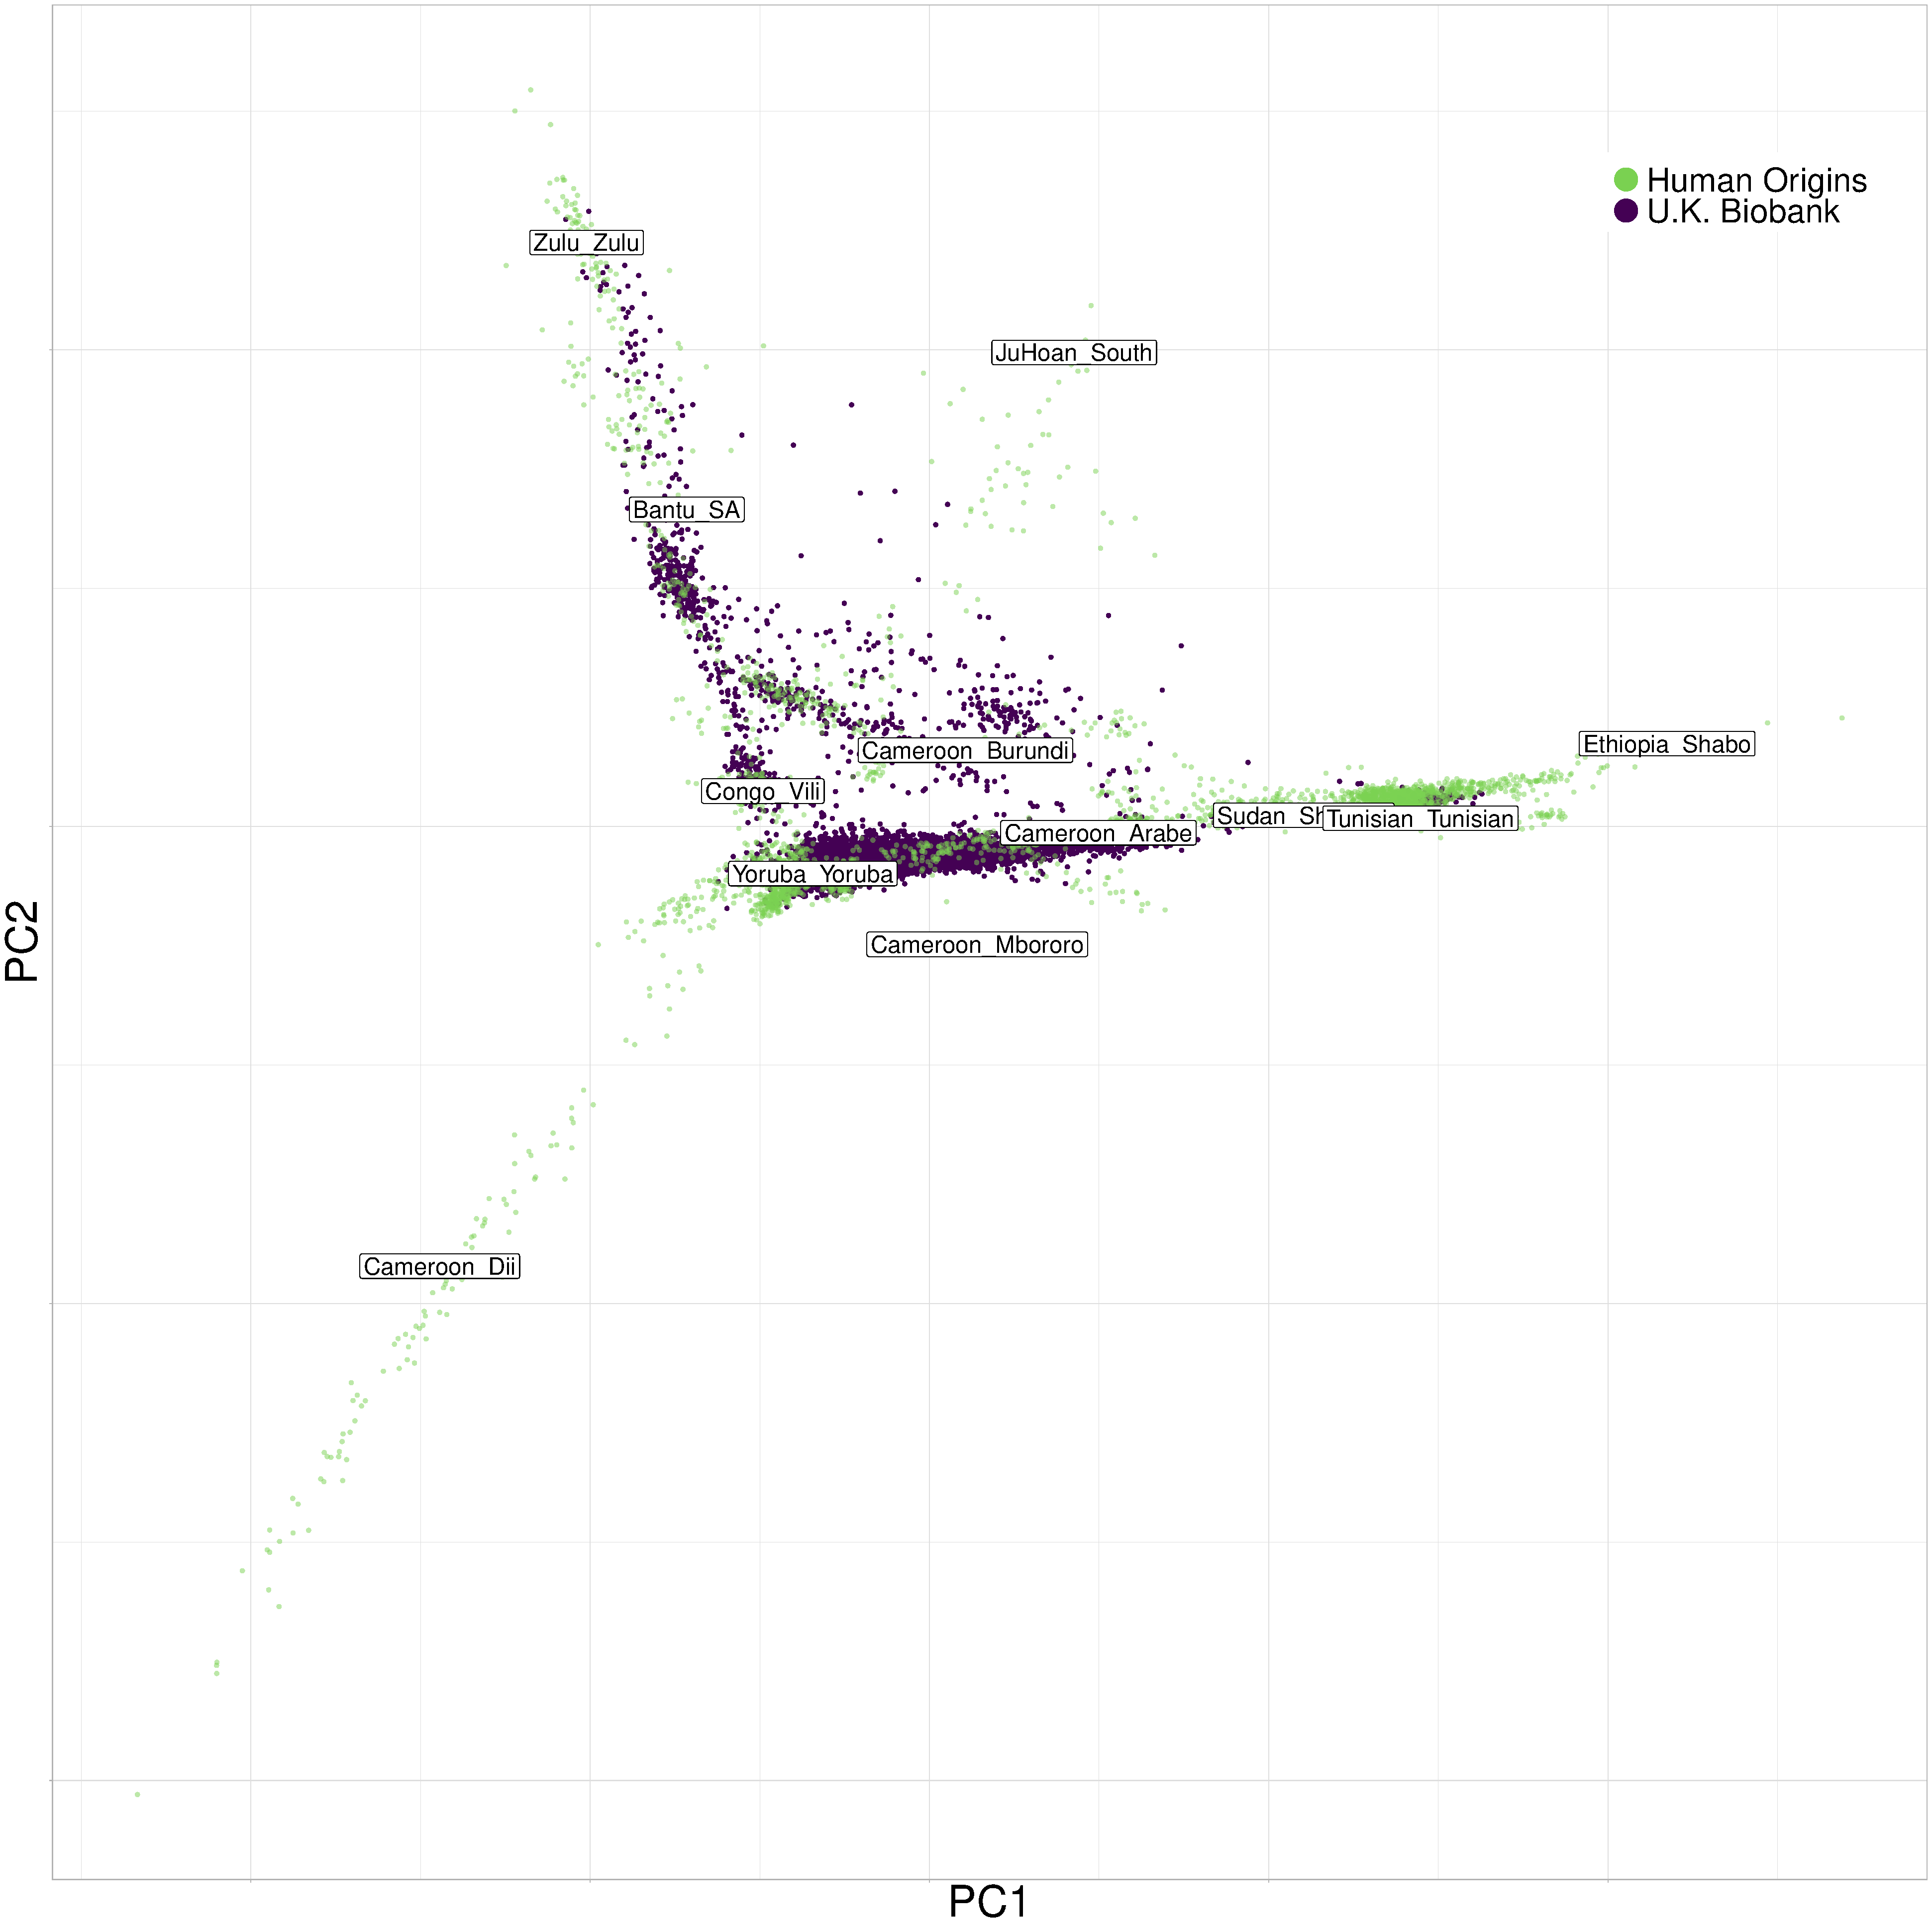
\includegraphics[width=1.0\textwidth]{../images/chapter3/ChromoPainter_PCA_UKB_HO.pdf}
    \caption{Principle component analysis of chunklengths matrix for all African UK Biobank individuals and human origins array. Individuals are coloured dependent on whether they are UK Biobank (green) or Human Origins (purple) samples. Labels indicate mean principle component coordinates for individuals in that population. A random sample of populations were chosen to have labels to prevent the figure from being too cluttered.}
    \label{fig:PCA_chunklengths_HumanOrigins_UKBiobank}
\end{figure}

Aggregating the columns of the aforementioned co-ancestry matrix by reference population by mean/sum gives the total length of genome that donor population has contributed to the selected U.K. Biobank individuals. This can be visualised on a map, where each point represents a reference population and the colour corresponds to the total amount that reference population contributes towards the ancestry of all retained UK Biobank individuals (Fig. \ref{fig:haplotype_sharing_map_zoomed_II}).

\begin{figure}[htp]
    \centering
    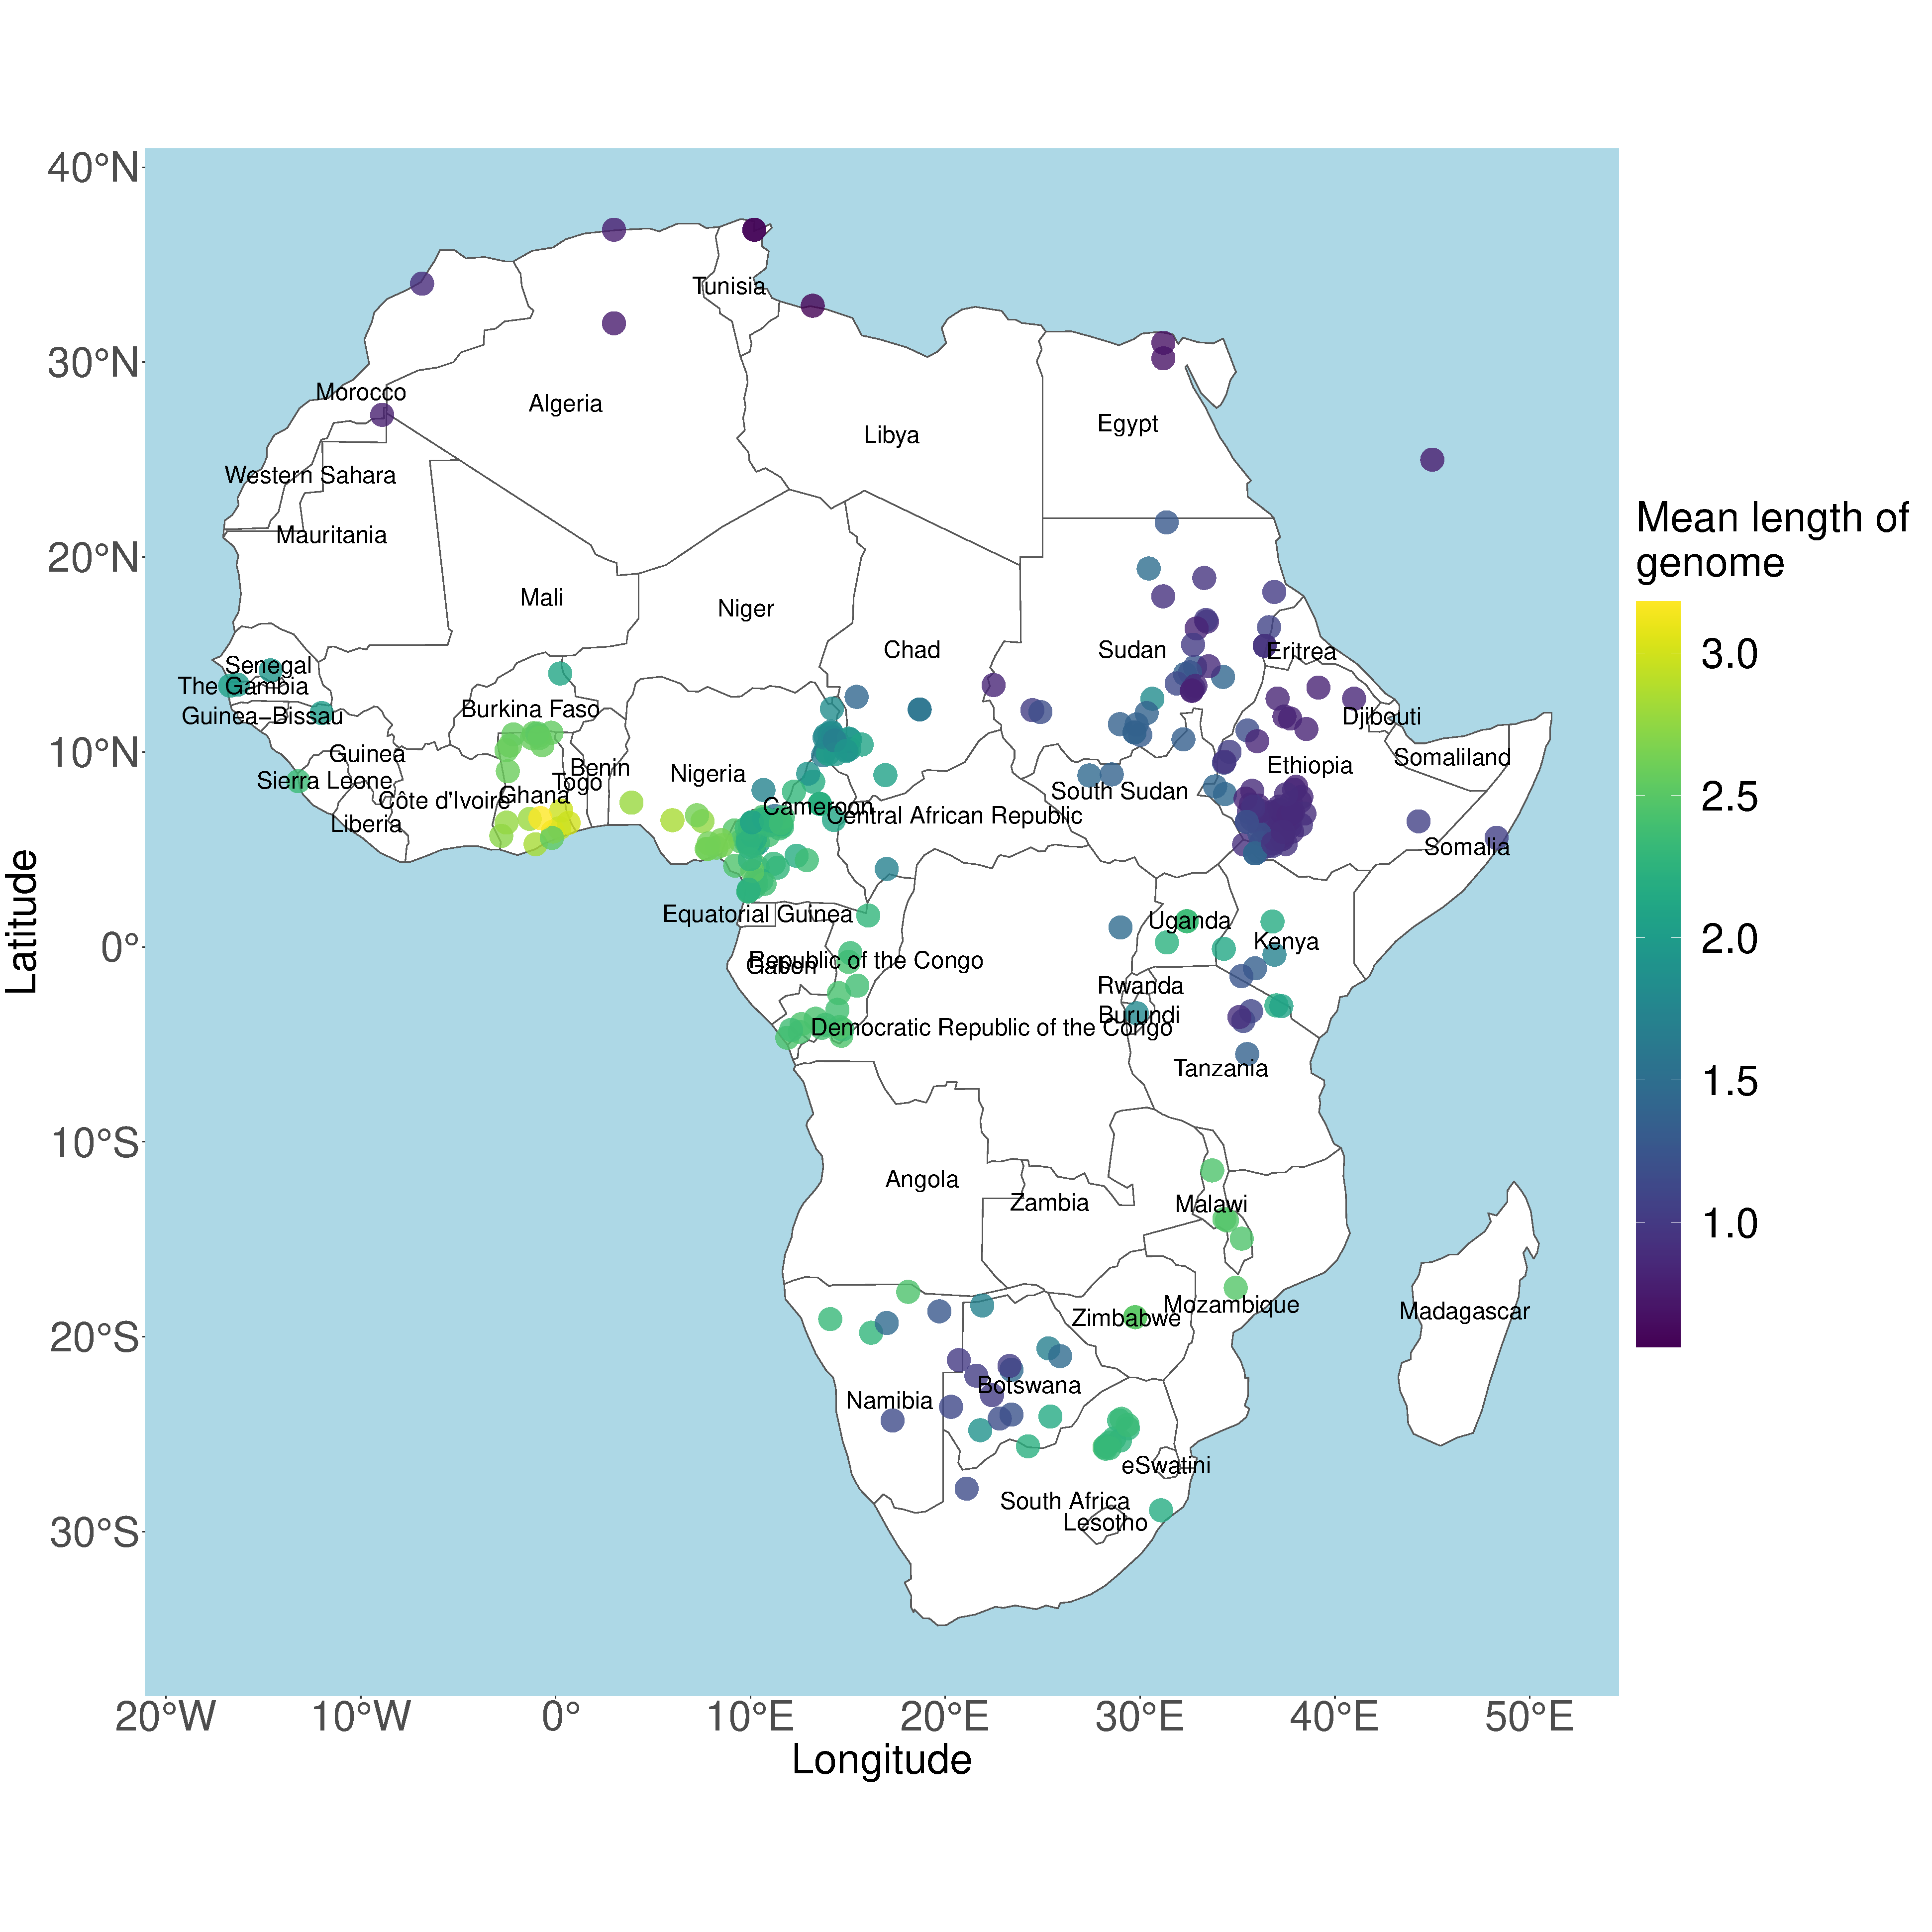
\includegraphics[width=1.0\textwidth]{../images/chapter3/haplotype_sharing_map_zoomed_II.pdf}
    \caption{Map of haplotype donation to UK Biobank individuals. Each point represents a different African population. Colour }
    \label{fig:haplotype_sharing_map_zoomed_II}
\end{figure}

The populations with the largest contribution to the retained UK Biobank samples are those from West Africa. This is consistent with two different historical processes. 

Firstly, it is known from historical and genetic studies that a majority of the individuals who were forcibly transported from Africa to the Americas during the transatlantic slave trade were from the west coast of Africa \cite{micheletti2020genetic}. Given the UK Biobank sample contains many individuals who were either born in, or trace their ancestry from the Caribbean, we would expect there to be a large contribution of ancestry from West Africa.

Secondly and more recently, there has been a relatively large amount of historical immigration from countries in West Africa, such as Ghana and Nigeria, to the U.K. 

\subsection{Verifying painting accuracy}

Given the total number of SNPs used in the analysis (n=65,727) is on an order of magnitude less than is typically used in such analysis, it is important to verify the results do not simply correspond to copying the most from the reference populations with the largest sample size, as has been shown in previous analyses (refer to previous chapters). To test that the coancestry matrix contains relevant information about the ancestry of the retained UK Biobank individuals, I took advantage of the UK Biobank metadata and subsetted the coancestry matrix to contain only individuals who were born in a particular country. We would expect that individuals who were born in a particular country would copy the most from reference populations from that country. For example, we would expect individuals who were born in South Africa to copy the most from Bantu and Zulu ethnic groups from South Africa. 

\begin{figure}[htp]
    \centering
    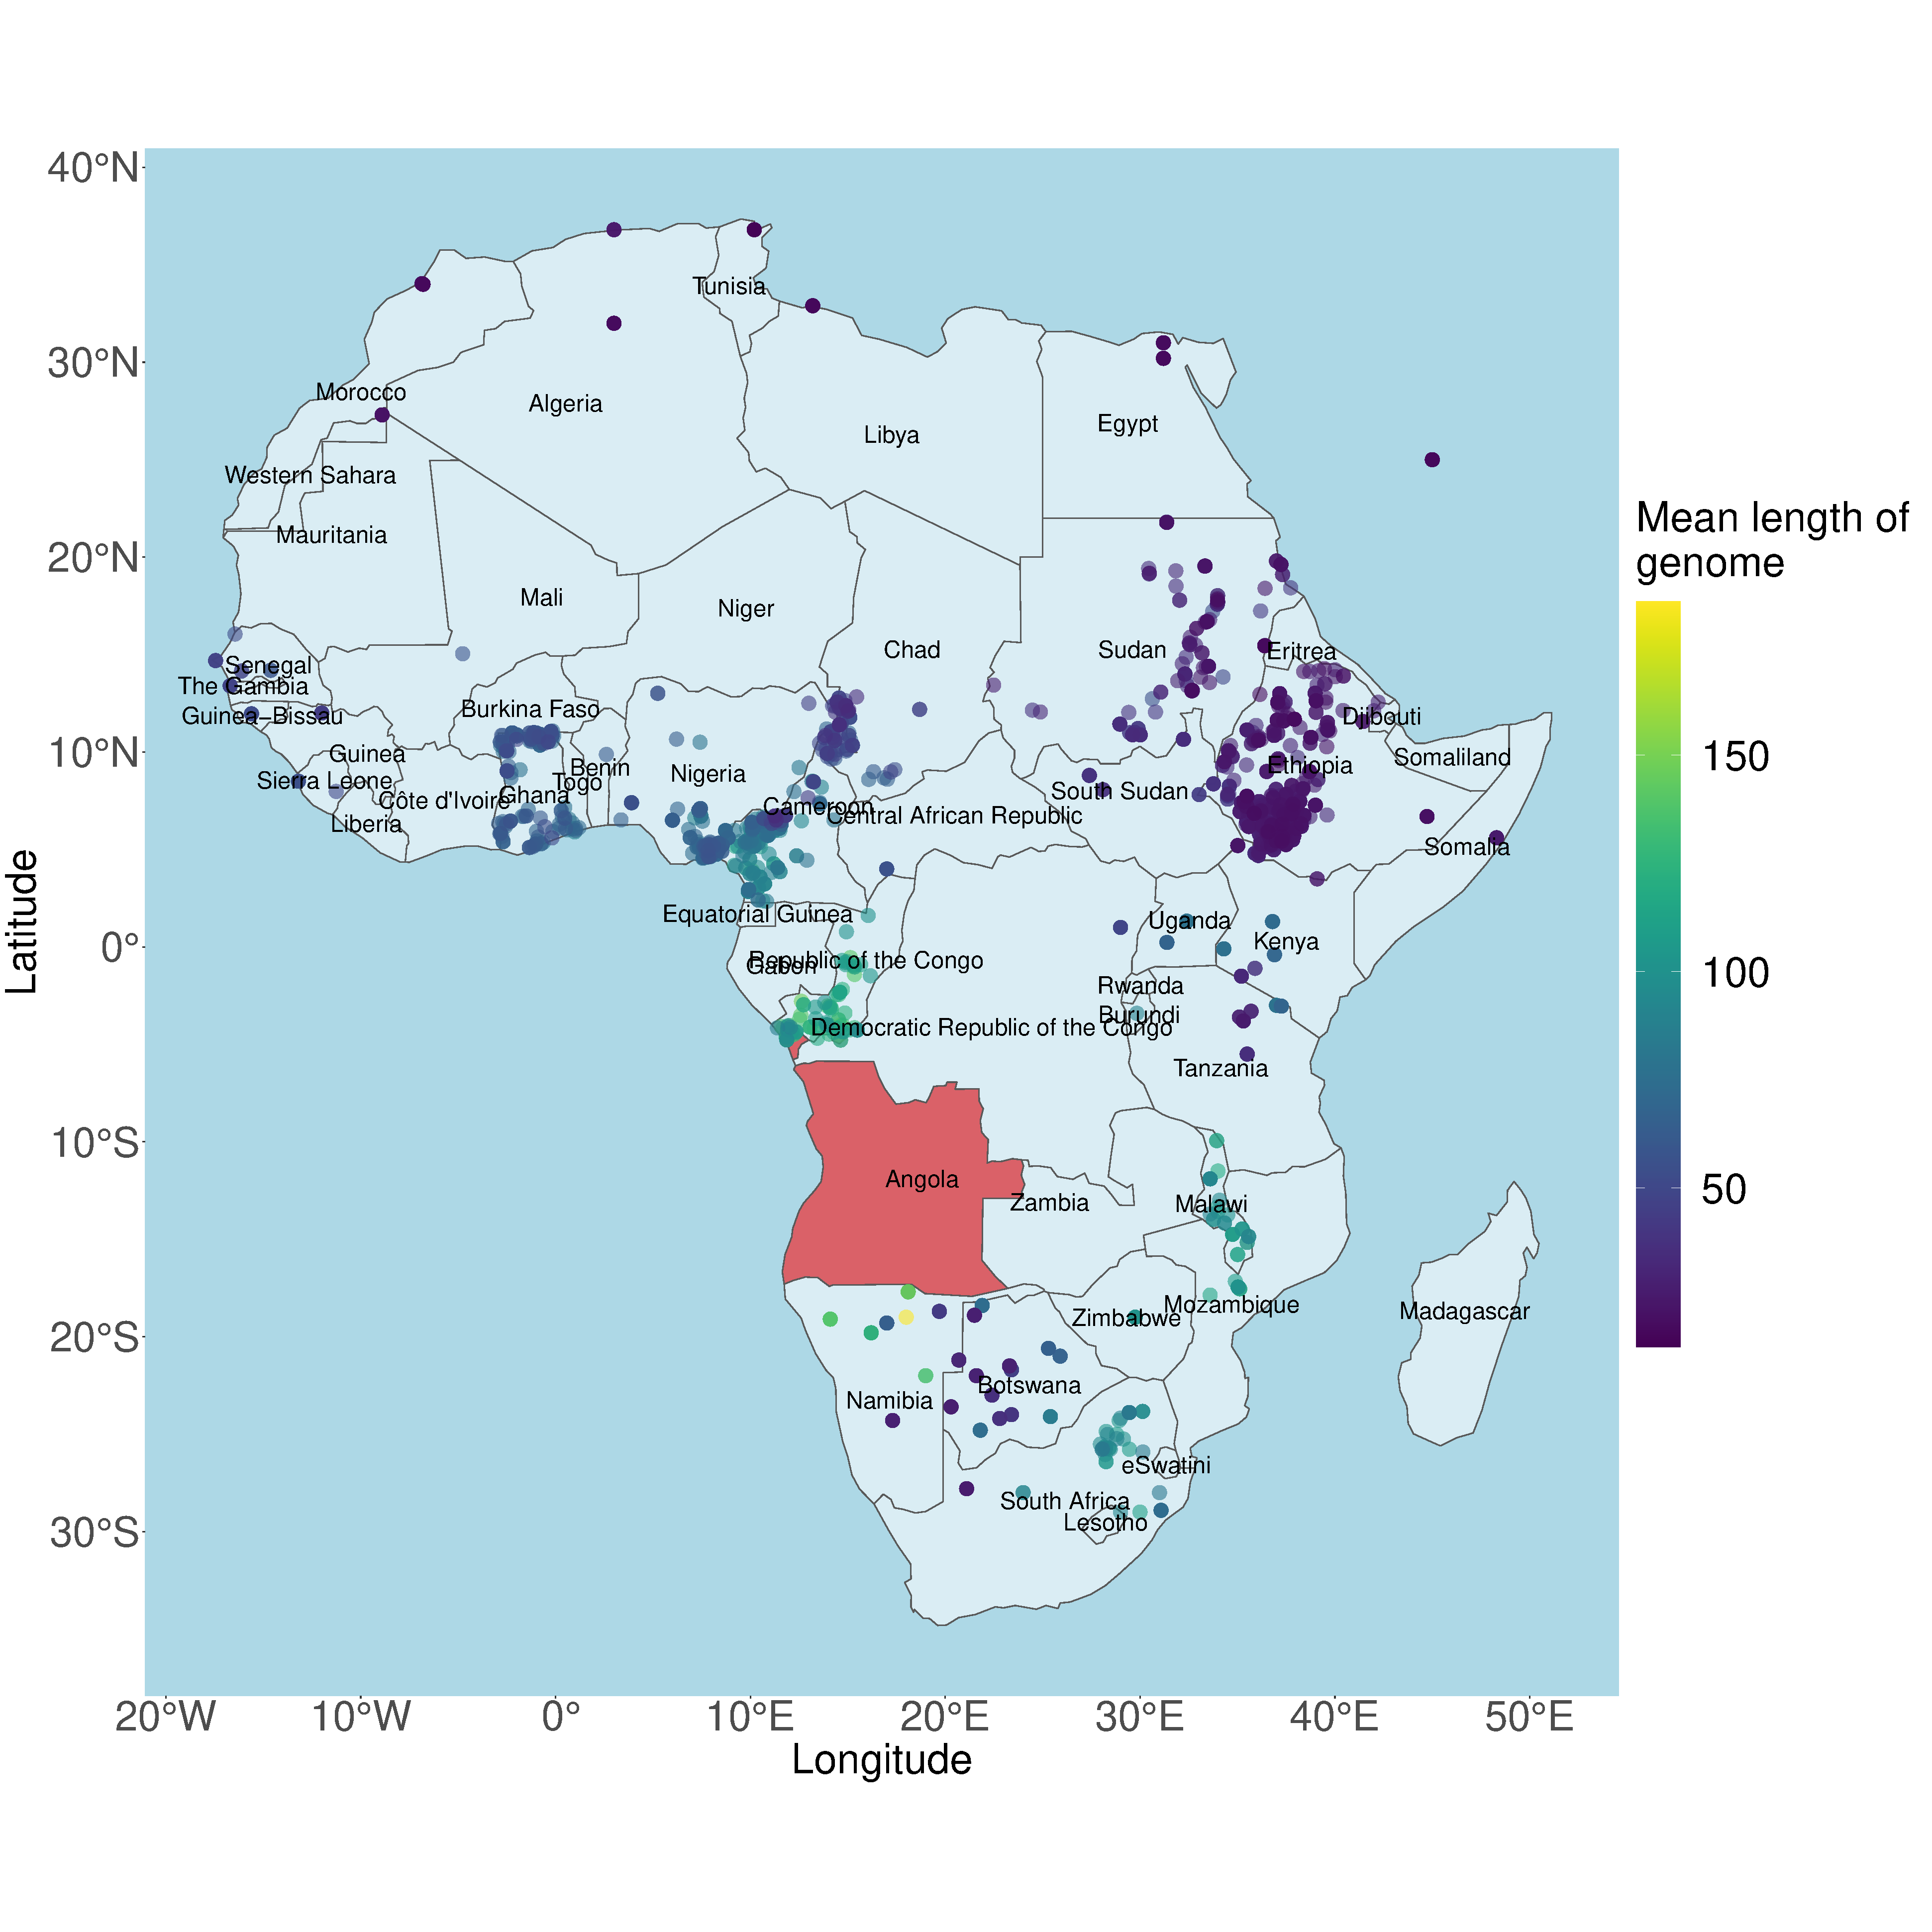
\includegraphics[width=1.0\textwidth]{../images/chapter3/haplotype_map_SouthAfrica.pdf}
    \caption{Map of haplotype donation to UK Biobank individuals born in South Africa.}
    \label{fig:haplotype_map_South Africa}
\end{figure}

Fig. \ref{fig:haplotype_map_South Africa} shows the map of haplotype donation from reference groups to UK Biobank individuals born in South Africa. It is clear that reference populations from South Africa, in particular the Zulu ethnic group, contribute the most to these individuals. The same pattern is clear for most countries of origin. 

There are several interesting cases. For example, there are N individuals who were born in the Caribbean. Visualising the haplotype donation map for these individuals shows that they are primarily of West African ancestry, consistent with historical evidence \cite{micheletti2020genetic}. Individuals born in Brazil have ancestry from further South, again consistent with historical evidence (citation needed).

As a more formal test of the painting accuracy, I estimated SOURCEFIND ancestry proportions in each retained UK Biobank individuals. An individual was 'assigned' to a particular reference population if they had 75\% or more ancestry from that population. If the country the assigned reference population is from matches the birth location of the individual, then I considered that a 'success' and a 'fail' otherwise. Individuals who were born in the U.K. or who had no birth country were excluded from this analysis. 

\begin{figure}[htp]
    \centering
    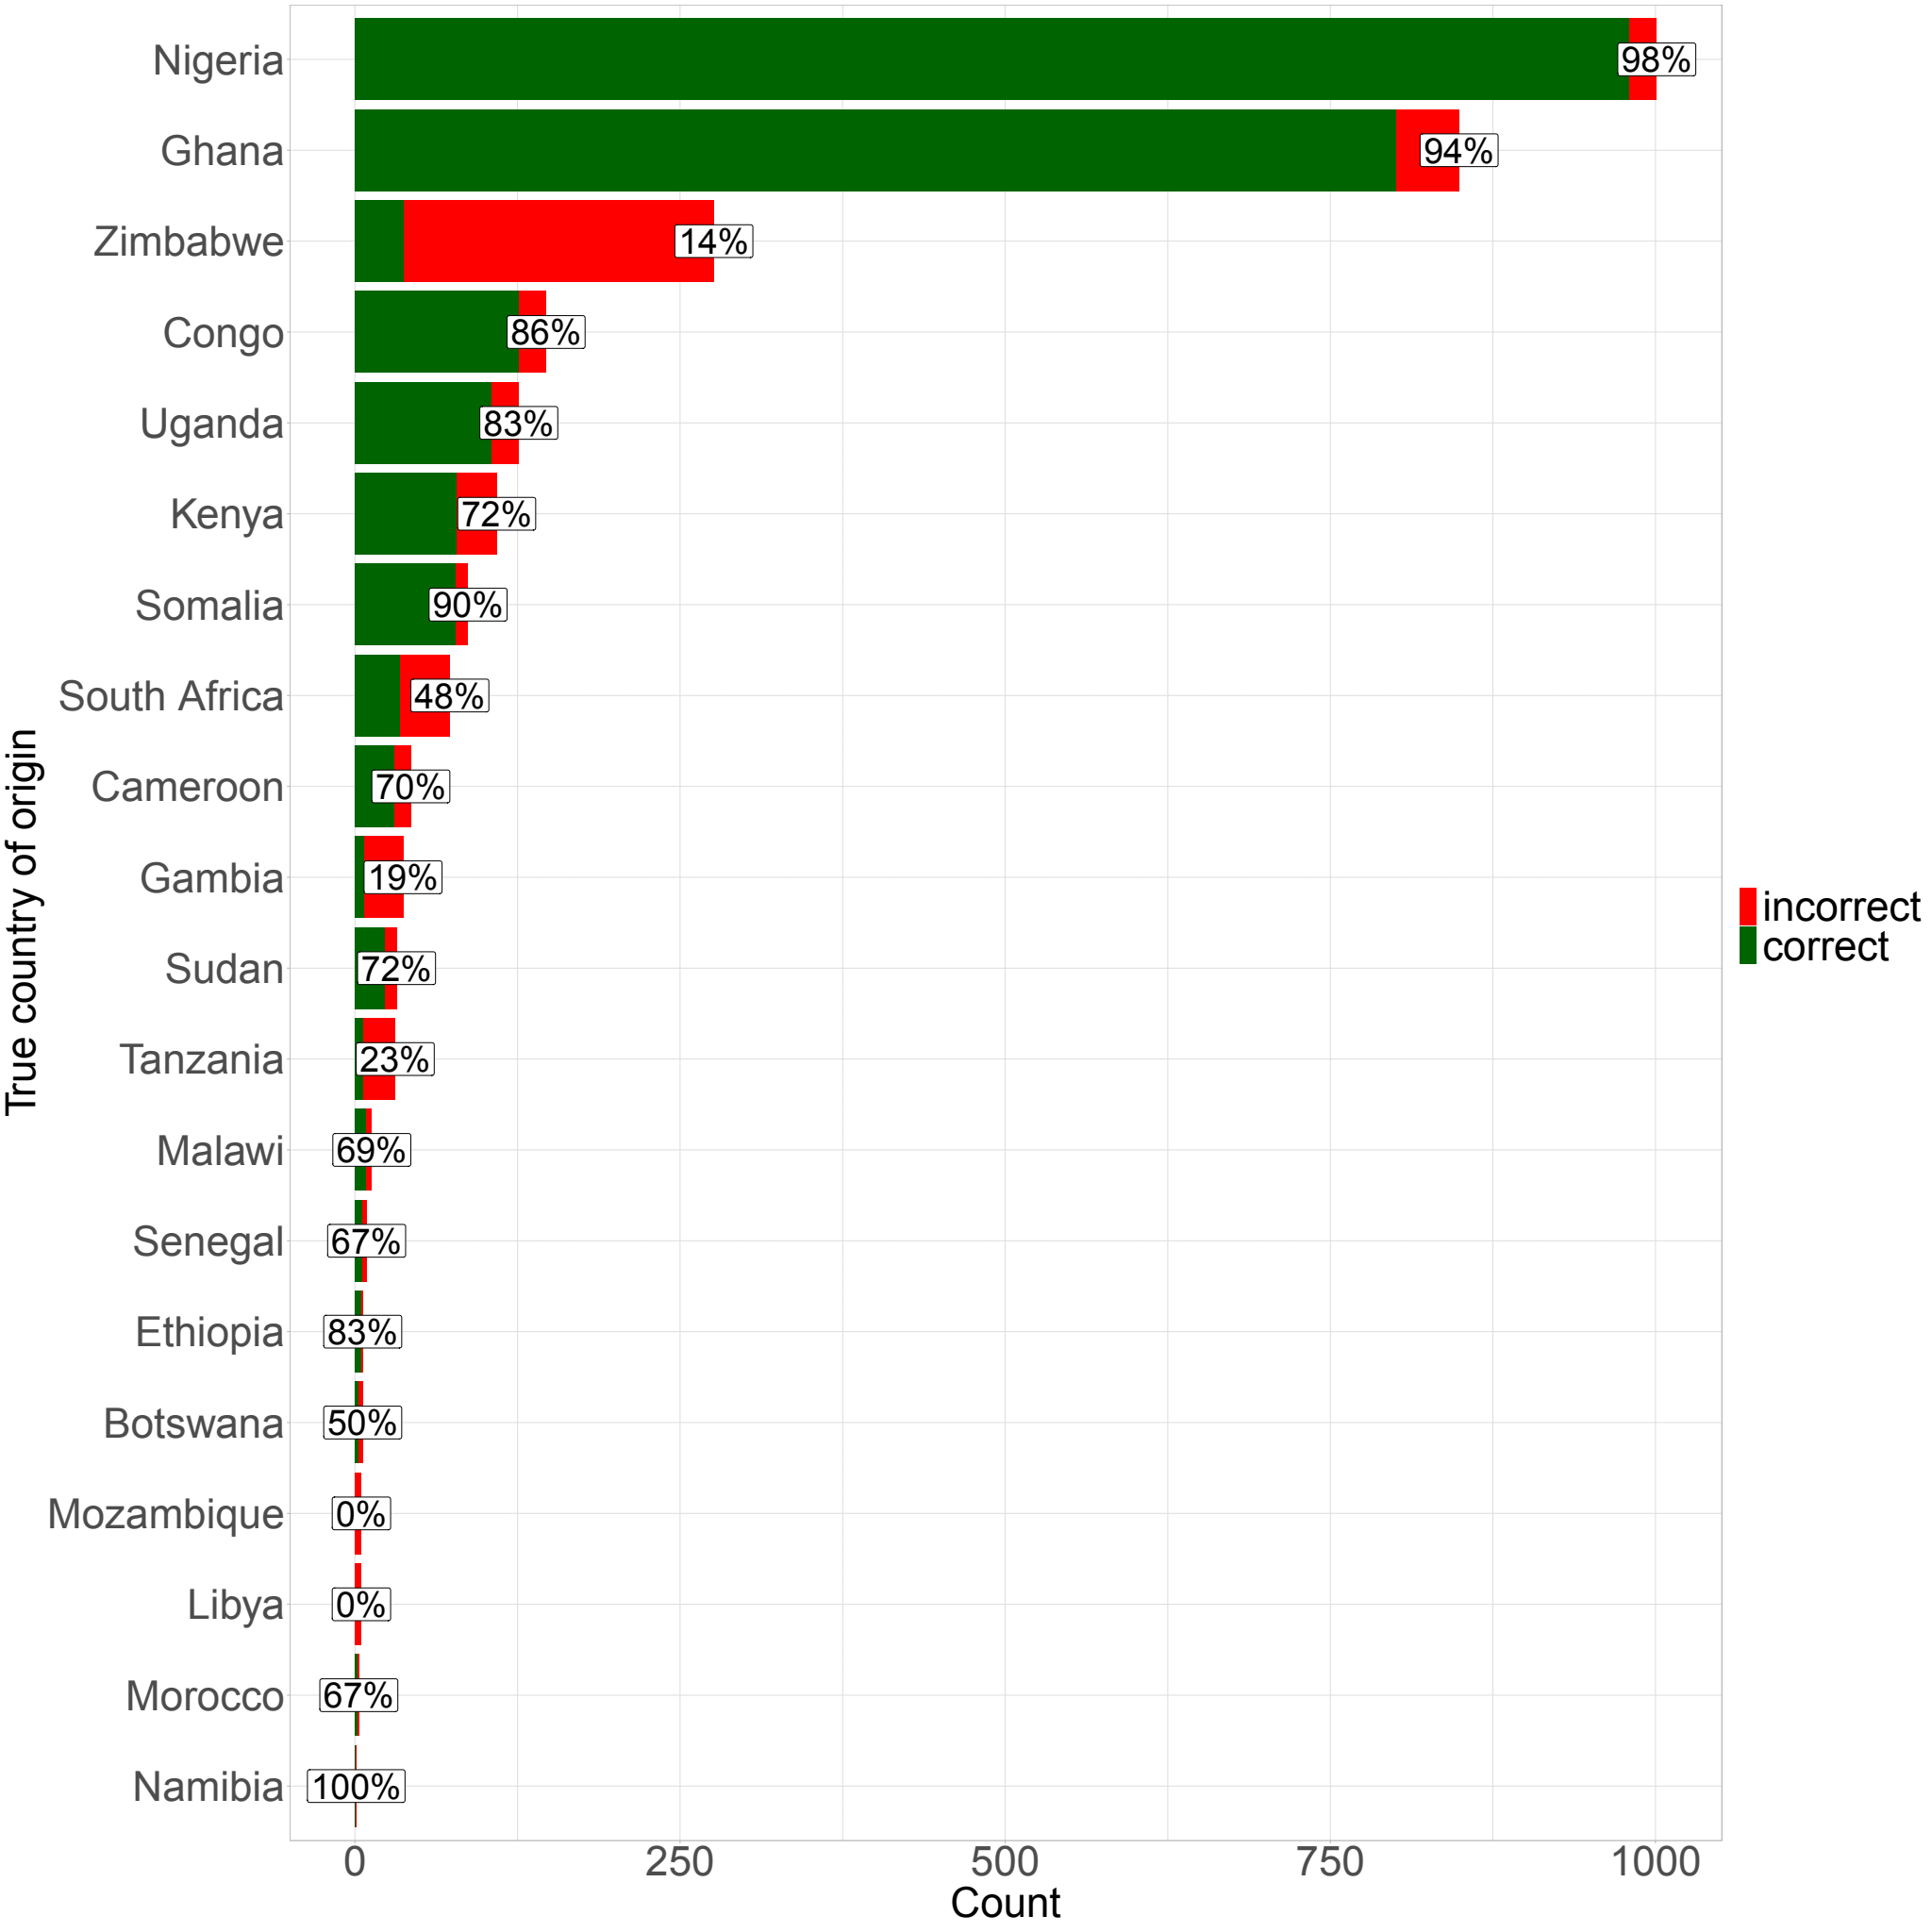
\includegraphics[width=1.0\textwidth]{../images/chapter3/country_of_origin_allInds.png}
    \caption{Correspondence of true birth country with estimated birth country. Each bar corresponds to a true birth country, with the length of the bar corresponding to the total number of people in our dataset born in that country. The green section corresponds to the total number of individuas where the birth country was correctly guessed and the red section to those who were incorrectly guessed. Percentage labels give percentage correct for that country.}
    \label{fig:country_of_origin_allInds}
\end{figure}

The overall accuracy at predicting birth location was 81.63\%, suggesting there was substantial information within the coancestry matrix. For the countries where there was a large number of reference populations, such as Ghana and Nigeria, the prediction accuracy was high. For certain countries, the prediction accuracy was much lower. For example, Tanzania was only represented by a single reference population. Zimbabwe...

I also wanted to perform the same analysis but using the data which had been imputed. This stands as a practical test of whether it is preferable to impute or retain a smaller number of non-imputed SNPs. 

\subsection{Imputation bias}

The imputed dataset consisted of 535,544 SNPs in total, 87.7\% of which were imputed. Having a high percentage of imputed SNPs may bias downstream analyses. 

For example, consider two UK Biobank individuals who have a large percentage of African ancestry. One of the individuals has ancestry relating to a particular Nigerian ethnic group and the other to a closely related, but different Nigerian ethnic group. We are interested in being able to determine the fine-scale differences in ancestry between these individuals. This relies on the existence of variants in each individual which are specific to that population.

Imputation relies on identifying reference haplotypes which are closest to the target haplotypes. However, neither of the ethnic groups that the individuals derive ancestry from are present in the imputation reference panel. Therefore, we would expect that the missing variants would be imputed from the populations in the reference panel which are most closely related to our target samples. In the case of the Haplotype Reference Consortium, the closest reference population to our two target samples may be the Yoruba. If missing are preferentially imputed from Yoruban individuals, then we would expect segments of the target samples to appear to me more 'Yoruba-like' than otherwise. Correspondingly, when painted using a reference panel which includes, but is not exclusive to, those populations found in the imputation reference panel, we would expect the populations found in the imputation reference panel to donate more.

Comparing the imputed and non-imputed coancestry matrices revealed biases consistent with the above expectation. If the coancestry matrix columns are combined into populations, then the sum of each column gives the total length of genome that population contributes to all recipient individuals in the dataset. Therefore, comparing the column sums between the imputed and non-imputed matrices informs us about which populations contribute more under in the imputed dataset than the non-imputed dataset. 

 \begin{figure}[htp]
    \centering
    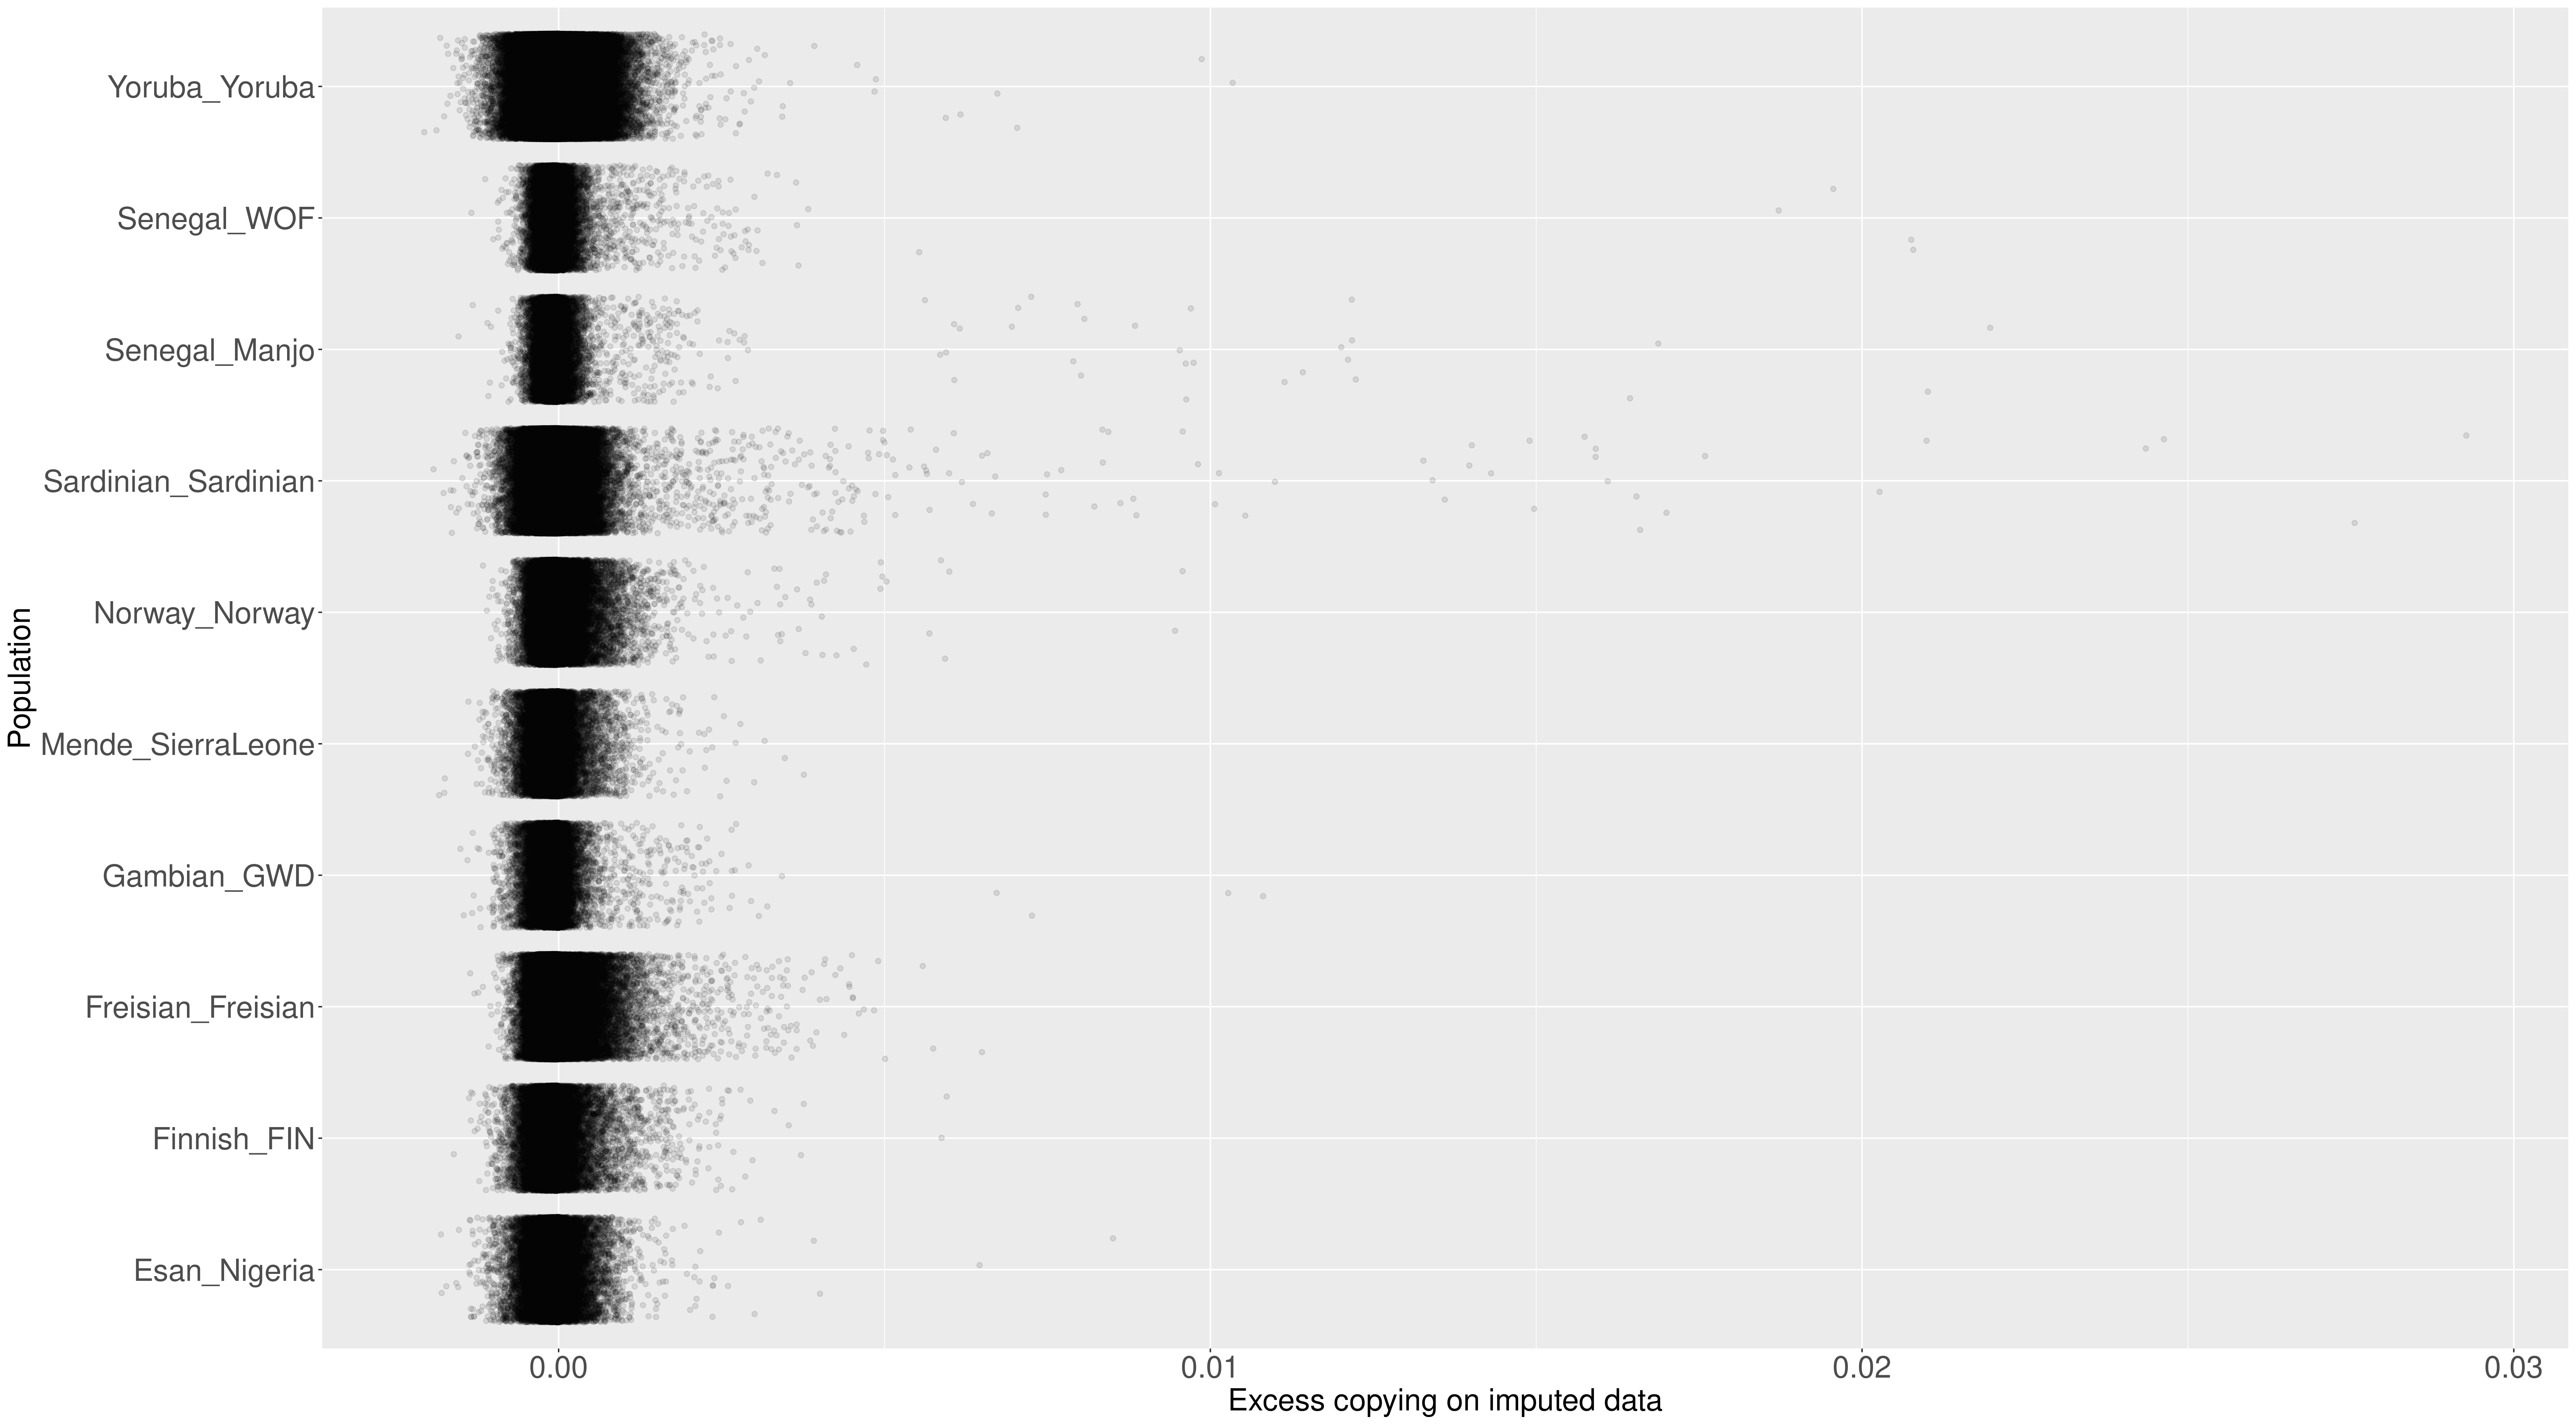
\includegraphics[width=1.0\textwidth]{../images/chapter3/imputed_excess_copying_pops.png}
    \caption{The top 10 Human Origins populations which donate more haplotypes under when data is imputed compared to non-imputed. Each point corresponds to the difference between the amount an individual from that donor population donated using imputed and non-imputed data, with positive values corresponding to more copying when the is imputed.}
    \label{fig:imputed_excess_copying_pops}
\end{figure}

Of the 568 populations tested, 6 were present in the 1000 genomes reference panel. 

Considering the SOURCEFIND results shows strong evidence that imputation alters the inferred ancestry proportions of the Human Origins individuals. If we take each target population and assign the surrogate with the largest ancestry proportion as the 'best surrogate', then only 30\% (144/478) of the best surrogates match between the imputed and non-imputed datasets. 

\subsection{Comparing sparse genotype to imputation}









